% generated by src/r2/paper_assets (make_paper_assets.py figures); do not edit by hand
% provenance: fig6_governance generated by src/r2/paper_assets on 2026-10-15 04:07 from data/r2/tables/
%   gov_tiers.csv (modified 2026-10-14 20:11): scope = dual, tier in {Strong, Moderate, Conditional}; draw interval columns
%   gov_tier_validation.csv (modified 2026-10-14 20:11): universe = global (scope global_fit) or tissues (scope dual); tier in {Strong, Moderate, Conditional}; reference in {encode, enets2, pert_pooled}
%   gov_promoted_by_method.csv (modified 2026-10-14 20:11): k = 50 (method top-k per TF) and method = all_edges
%   (constants): topk_per_tf from r2.common.PRESPECIFIED; MIN_CLUSTERS from r2.governance
\begin{figure}[tbp]
  \centering
  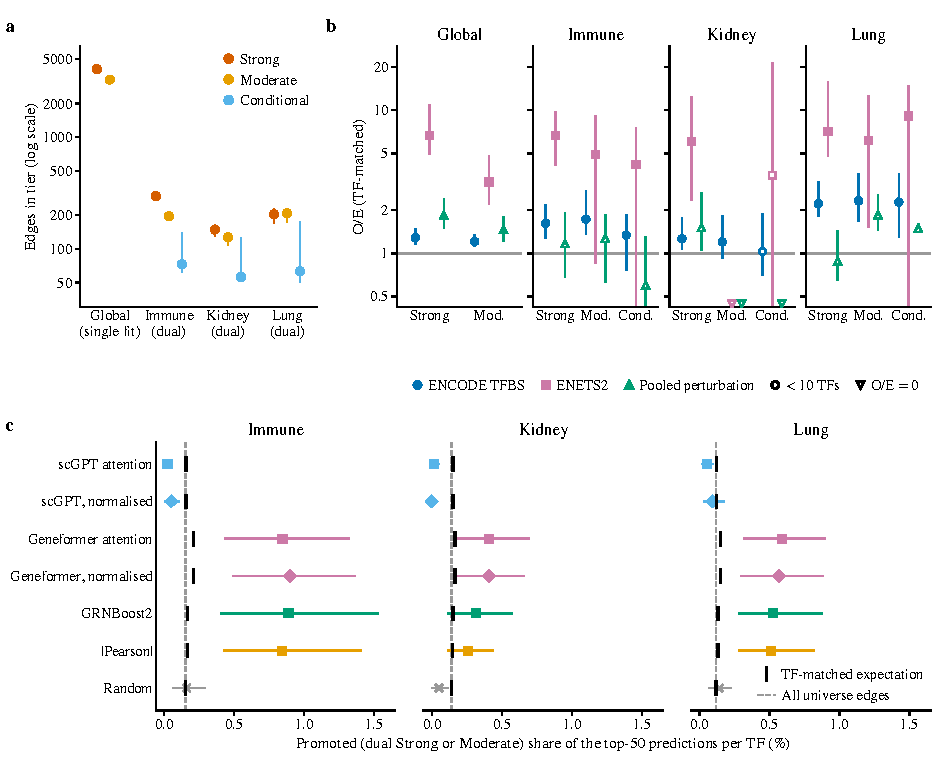
\includegraphics[width=\textwidth]{fig6_governance.pdf}
  \caption{\textbf{Claim governance.} (a) Number of edges per tier: single-fit BFDR tiers in the global universe (Strong 4{,}060, Moderate 3{,}274) and dual-universe tiers in the tissue universes (Strong/Moderate/Conditional: immune 297/196/73; kidney 149/127/56; lung 204/208/63), with 95\% intervals over posterior draws of the credibilities (tissue universes). (b) Held-out positives in each tier relative to the TF-matched expectation, with 95\% TF-bootstrap intervals (open markers: fewer than 10 evaluable TFs; triangles: no positive observed; intervals reaching 0 are cut at the axis). Global universe, Strong tier: ENCODE 1.29 [1.16, 1.48], ENETS2 6.67 [4.88, 10.95], pooled perturbation 1.85 [1.49, 2.43]; Moderate tier: 1.21 [1.11, 1.35], 3.16 [2.21, 4.80], 1.47 [1.21, 1.81]. (c) Share of each method's top-50 predictions per TF that are promoted (95\% TF-bootstrap intervals), against the share expected if the method picked random targets of the same TFs (bars) and the share among all universe edges (dashed). scGPT attention: immune 0.03\% vs 0.16\% expected; Geneformer attention: immune 0.85\% vs 0.21\% expected; GRNBoost2: immune 0.89\% vs 0.17\% expected.}
  \label{fig:governance}
\end{figure}
